\begin{figure}
	\centering
	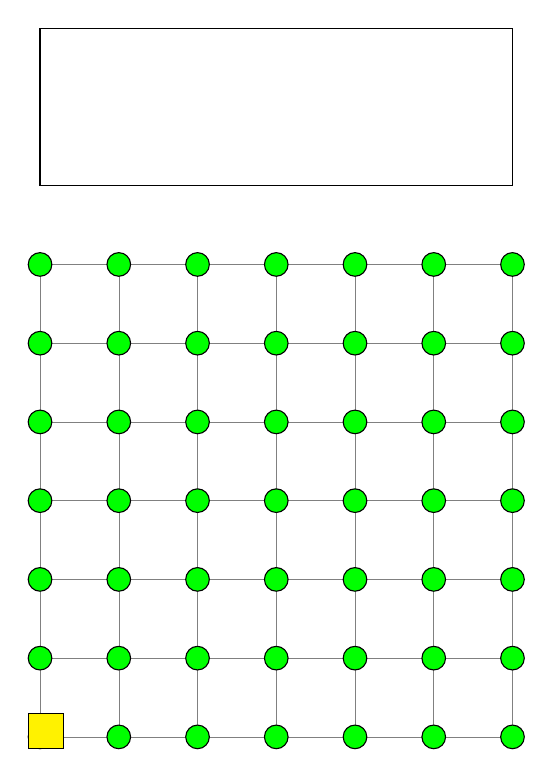
\begin{tikzpicture}[axis/.style={thin, black, ->, >=stealth'}]
	
		\def \nx {6}
		\def \ny {6}
		
	
		\draw (0, 7) rectangle (6,9);
		\draw[step=1cm,gray,very thin] (0,0) grid (\nx,\ny);
		\foreach \ix in {0,...,\nx}{
			\foreach \iy in {0,...,\ny}{
				\filldraw[fill=green] (\ix,\iy) circle (0.15);
			}
		}
		\filldraw[fill=yellow] (-0.15, -0.15) rectangle (0.3, 0.3);
%		\filldraw[fill=yellow] (0,0) circle (0.15);

	\end{tikzpicture}
	\caption{Caption}
	\label{fig:grid_of_nodes}
\end{figure}